% !TEX root = cas-dc-template.tex
%\documentclass[a4paper,fleqn,longmktitle]{cas-dc}
\documentclass[a4paper,fleqn]{cas-dc}

%\usepackage[authoryear,longnamesfirst]{natbib}
%\usepackage[authoryear]{natbib}
\usepackage[numbers]{natbib}
\usepackage{caption}
\usepackage{graphicx}
\usepackage{pifont}  
\usepackage{microtype}
\usepackage{siunitx}
%%%Author definitions
\def\tsc#1{\csdef{#1}{\textsc{\lowercase{#1}}\xspace}}
\tsc{WGM}
\tsc{QE}
\tsc{EP}
\tsc{PMS}
\tsc{BEC}
\tsc{DE}
%%%
         
\begin{document}
\let\WriteBookmarks\relax
\def\floatpagepagefraction{1}
\def\textpagefraction{.001}
\shorttitle{ISPRS Journal of Photogrammetry and Remote Sensing}
\shortauthors{Wei Jing et~al.}

\title [mode = title]{GOLD: Guided Online Learning for Distillation for Heterogeneous Remote Sensing Image Change Detection}

\tnotetext[1]{}

\author[1,2]{Wei Jing}
\ead{wei_adam@mail.nwpu.edu.cn}

\author[2]{Haichen Bai}
\ead {hcbai@mail.nwpu.edu.cn}

\author[2]{Binbin Song}
\ead {songbinbin@mail.nwpu.edu.cn}

\author[3]{Weiping Ni}
\ead {niweiping@nint.ac.cn}

\author[3]{Junzheng Wu}
\ead {wujunzheng@nint.ac.cn}

\author[2]{Qi Wang\corref{mycorrespondingauthor}}
\cortext[mycorrespondingauthor]{Corresponding author}
\corref{mycorrespondingauthor}
\ead{crabwq@gmail.com}

\address[1]{National Elite Institute of Engineering, Northwestern Polytechnical University, Xi'an 710072, China}
\address[2]{School of Artificial Intelligence, OPtics and ElectroNics (iOPEN), Northwestern Polytechnical University, Xi'an 710072, China}
\address[3]{Department of Remote Sensing, Northwest Institute of Nuclear Technology, Xi'an 710072, China}

\begin{abstract}
Given the inherent differences in imaging mechanisms, there exists a significant heterogeneity gap between heterogeneous remote sensing images. Effectively extracting surface change information from such heterogeneous data remains a core challenge for accurate monitoring of land cover dynamics. To address this, this paper constructs a Bi-temporal Multi-sensor Change Detection (BtMs-CD) dataset, aiming to guide the feature learning of synthetic aperture radar (SAR) data towards the representation paradigm of optical data. Based on this, we propose the Guided Online Learning with Knowledge Distillation (GOLD) model, which adopts a three-branch architecture. By leveraging a teacher network pre-trained on homogeneous optical data, the knowledge learned by the teacher network is transferred to the student network, which processes heterogeneous optical-SAR data. Specifically, we leverage multi-metric difference maps and spatiotemporal attention mechanisms to deeply mine discriminative change features, enabling precise extraction of surface change information. Subsequently, a difference-aware attention transfer mechanism is designed to drive cross-modal feature alignment, effectively bridging the representational gap between optical and SAR data. Finally, an adaptive dynamic weight allocation strategy is implemented to optimize the collaborative balance between knowledge transfer and change detection tasks, significantly enhancing the model's robustness and generalization ability in complex heterogeneous scenarios. Experimental results demonstrate that the proposed model outperforms existing state-of-the-art methods, achieving an IoU of 85.98\% on heterogeneous data, nearly matching the performance of the teacher network on homogeneous data (86.61\%). The model code and dataset can be found at: \href{https://github.com/Mriris/HeteroCD-GOLD}{https://github.com/Mriris/HeteroCD-GOLD}.
\end{abstract}



\begin{keywords}
Heterogeneous Remote Sensing Images, Change Detection, Online Knowledge Distillation, Difference Map Attention Transfer, Dynamic Weight Allocation
\end{keywords}


\maketitle

\section{Introduction}
By comparing multi-temporal observations of the same geographic region, change detection techniques can accurately identify and quantify surface dynamics. This capability is crucial for revealing the processes and assessing the extent and severity of phenomena such as urban expansion, deforestation, crop growth, and damage caused by natural disasters. In contrast, heterogeneous change detection (HCD) aims to overcome the limitations of single-source data by enabling more flexible, comprehensive, and, in some cases, the only feasible means of capturing and interpreting these changes.

Homogeneous change detection in remote sensing images typically relies on multi-temporal imagery acquired from the same platform and sensor. Such data exhibit highly consistent geometric structure, radiometric response, and spectral characteristics, which significantly reduce system errors and noise introduced by sensor discrepancies. This consistency enhances both the accuracy and interpretability of change detection results. However, in practical scenarios, stable acquisition of homogeneous remote sensing imagery is often constrained by factors such as weather conditions, imaging schedules, and sensor availability. These challenges are particularly pronounced in time-sensitive applications such as emergency response and military activity monitoring. To overcome the limitations associated with homogeneous data acquisition, HCD has emerged as a promising alternative. Its core objective is to extract reliable surface change information from multi-source remote sensing images characterized by substantial differences in imaging mechanisms—such as optical imagery and synthetic aperture radar (SAR) data. Although the large representational gap between heterogeneous data increases the complexity of feature alignment and change discrimination, HCD offers unique advantages in terms of data acquisition flexibility and cross-modality applicability. Therefore, it has become an important complementary approach for studying dynamic land cover changes.

Despite its significant potential in overcoming the limitations of single-source data, HCD still faces several critical challenges that hinder its effective implementation. These challenges are primarily reflected in the following aspects: (1) Interference from “pseudo-changes” caused by cross-domain discrepancies: Different sensors exhibit inherent differences in imaging mechanisms, spatial resolution, spectral response functions, and atmospheric conditions. As a result, even when no actual surface change has occurred, the same ground object may present substantially different—and often nonlinear—appearances across heterogeneous images. This leads to the generation of a large amount of pseudo-change noise that is unrelated to real surface changes, severely impacting the accuracy of true change extraction. (2) Difficulty in disentangling change features from sensor-specific differences: Under conditions of strong domain shifts, HCD models must possess powerful feature representation capabilities to extract deep semantic features that are invariant to sensor-related discrepancies while remaining sensitive to actual surface changes. Designing model architectures and optimization mechanisms that can adaptively suppress inter-domain variations while effectively capturing and enhancing true change signals remains a core technical challenge. (3) Lack of high-quality annotated datasets: Currently, there is a shortage of HCD datasets that offer both high-precision spatiotemporal alignment and authoritative “gold standard” annotations. This limitation introduces uncertainty into model training and performance evaluation, due to label noise and annotation bias. To address these issues, there is an urgent need to develop more robust domain adaptation and feature alignment strategies, refined change modeling mechanisms, and rigorous evaluation protocols to enhance the accuracy and applicability of heterogeneous change detection in real-world scenarios.

To address the aforementioned challenges, we systematically construct BtMs-CD, the first bi-temporal multi-sensor change detection dataset. This dataset integrates pre-event high-resolution optical imagery, post-event synthetic aperture radar (SAR) imagery, and post-event optical imagery, with precise pixel-level annotations. BtMs-CD focuses on the dynamic evolution of buildings in urban–rural fringe areas during urbanization processes, accurately capturing two core types of structural changes: newly constructed and demolished buildings. Based on this carefully curated dataset, we propose a novel heterogeneous change detection framework named GOLD, driven by homogeneous-domain knowledge distillation. The core design of GOLD aims to efficiently model and disentangle complex change patterns embedded in highly heterogeneous remote sensing data. Specifically, GOLD adopts a teacher–student distillation architecture, where the teacher network learns high-level semantic representations from homogeneous optical image pairs. These representations are then used to guide and constrain the student network, enabling it to align feature distributions effectively across heterogeneous modalities (i.e., optical and SAR domains). Thanks to this collaborative mechanism, the GOLD framework can robustly identify and localize changed building structures during inference. Extensive quantitative evaluations conducted on the BtMs-CD dataset demonstrate that GOLD achieves superior performance, significantly outperforming state-of-the-art change detection methods. The main contributions of this work are summarized as follows:

1) A high-quality dataset named BtMs-CD is introduced to advance research in change detection. This dataset consists of pre-disaster optical images, post-disaster synthetic aperture radar (SAR) images, and post-disaster optical images, with precise manually annotated building change instances.

2) By leveraging multi-metric difference maps and a difference-aware attention transfer mechanism, the proposed approach accurately captures surface change information while promoting cross-modal feature alignment, effectively narrowing the feature gap between optical and SAR data.

3) A knowledge distillation-based Guided Online Learning via Distillation (GOLD) model is developed. In this framework, homogeneous change knowledge learned by the teacher network is transferred to a student network that operates on heterogeneous optical-SAR data, enabling robust extraction of change instances. Extensive experiments conducted on the BtMs-CD dataset demonstrate the effectiveness and generalizability of the proposed GOLD model.
\section{Related work}
Remote sensing image change detection involves comparing and analyzing remote sensing images acquired from the same spatial location but at different time periods to determine whether changes have occurred in a specific ground area \cite{B01}. With the rapid advancement of remote sensing technology, change detection applications have achieved substantial progress and have been extensively utilized in domains such as disaster management, environmental monitoring, and urbanization \cite{B02}.

In the event of natural disasters, rescue personnel require timely insights into the disaster's extent and efficient assessments of affected regions to execute effective emergency response and recovery operations. Remote sensing change detection techniques can analyze multi-temporal images to identify surface alterations, thereby providing critical information for post-disaster evaluations. Following the 2023 Turkey-Syria earthquake, researchers employed Sentinel-2 optical images and Sentinel-1 synthetic aperture radar (SAR) images for change detection, enabling rapid assessments of damage to buildings and roads to support rescue efforts \cite{B03}. Domain experts have leveraged Sentinel-1, Sentinel-2, and Landsat-9 images to identify victims and infrastructure in flood scenarios, thereby enhancing flood mapping for the design of efficient mitigation strategies \cite{B04}. In environmental monitoring, remote sensing change detection facilitates the tracking of land cover variations, deforestation, and water quality changes, offering a scientific foundation for environmental protection policies [5,6]. Scholars have also utilized Sentinel-2 optical images in conjunction with Sentinel-1 SAR images for mapping deforestation losses \cite{B07}. In urban planning, change detection technology monitors urban expansion, infrastructure development, and land use transformations, supplying essential data for sustainable urban development strategies \cite{B08}.

Owing to the growing diversity and enhanced precision of satellite sensors, remote sensing images now serve as reliable data sources for investigating urban expansion and intra-urban dynamics. However, high-resolution remote sensing images often exhibit highly complex and diverse surface characteristics, along with substantial noise. Consequently, for features with subtle appearance differences—such as vegetation, soil, and water bodies—both SAR and high-resolution optical images present similar visual traits and significant noise, posing considerable challenges to traditional change detection methods \cite{B09}. Thus, enhancing the efficiency of heterogeneous remote sensing image change detection has emerged as a prominent research focus \cite{B10}.

\subsection{Homogeneous Change Detection}
Homogeneous remote sensing image change detection entails utilizing data acquired from sensors with identical or comparable imaging principles, such as change detection between SAR images or between optical images. Given that homogeneous remote sensing images share similar spectral and imaging mechanisms, detection can be performed directly based on the images' spectral and textural features \cite{B11}.

Homogeneous remote sensing image change detection methods have undergone rapid evolution, yielding numerous advanced techniques, including algebraic approaches (e.g., image differencing and ratio analysis), classification methods (e.g., supervised and unsupervised classification), and object-oriented methods \cite{B12}. As homogeneous images occupy similar feature spaces, straightforward linear operations suffice to generate change maps.

Homogeneous remote sensing image change detection demonstrates notable advantages in monitoring building alterations, road network expansions, and variations in urban green space areas during urban growth assessments \cite{B13}. Volpi et al. investigated a supervised method based on support vector machine classifiers for detecting changes in high-resolution images \cite{B14}. Peng et al. proposed an end-to-end neural network-based change detection approach for semantic segmentation, accompanied by the creation of a dedicated dataset for network training \cite{B15}.

Nevertheless, homogeneous remote sensing image change detection is not without limitations; for instance, commonly used optical sensors are susceptible to external factors such as weather and sunlight, resulting in inconsistent image quality \cite{B16}. With the proliferation of diverse satellite sensor types, homogeneous image-based change detection increasingly falls short of practical requirements, particularly in scenarios where such images are unavailable \cite{B17}.

\subsection{Heterogeneous Change Detection}
Heterogeneous remote sensing image change detection involves employing images captured by sensors with disparate imaging modalities, such as combinations of SAR and optical images. In contrast to homogeneous approaches, pixels in heterogeneous images reside in distinct feature spaces, rendering change maps unobtainable through simple linear operations or other homogeneous techniques—a primary challenge in this domain \cite{B18}.

In recent years, the development of various satellite sensors has rendered the application of heterogeneous remote sensing images increasingly vital in change detection \cite{B12}. Constraints imposed by technology, timing, or atmospheric conditions often limit access to archived optical images in emergency contexts, compelling researchers to rely on heterogeneous images for detection \cite{B19}. During the 2020 Australian bushfires, smoke and cloud cover necessitated the use of post-disaster SAR images for assessments \cite{B20}. Consequently, the advancement of novel change detection technologies tailored for heterogeneous images holds substantial importance.

Presently, beyond optical images, SAR images represent the most prevalent type in remote sensing. Optical images are derived from the reflection of sunlight on various objects, facilitating ease of acquisition and interpretation, albeit subject to the aforementioned limitations of optical sensors \cite{B16}. SAR images quantify the reflectivity of ground targets, remaining unaffected by environmental conditions and enabling all-weather, all-time monitoring; however, due to range-dependent imaging and multiple signal reflections, they are comparatively abstract and challenging to interpret \cite{B21}. Heterogeneous pairs comprising optical and SAR images are complementary, encompassing richer information than pairs of solely SAR or optical images \cite{B11}. Accordingly, images from all-weather SAR sensors can be integrated with pre-disaster optical images for comparative analysis, facilitating comprehensive disaster impact evaluations \cite{B22}.


\section{METHODOLOGY}
\subsection{Overall Framework}
GOLD (Guided Online Learning for Distillation) is a three-branch architecture specifically designed for heterogeneous remote sensing change detection. Unlike conventional dual-branch models, GOLD introduces a teacher–student framework that leverages relatively easy homogeneous change detection to guide the more challenging heterogeneous task. As illustrated in Fig.~\ref{fig:model_framework}, the model consists of three branches: a shared pre-event optical branch, a post-event optical branch (teacher), and a post-event SAR branch (student). The teacher network $T$ is responsible for optical–optical detection, while the student network $S$ handles optical–SAR detection.

Given a pre-event optical image $X_{pre}^{opt}$, a post-event optical image $X_{post}^{opt}$, and a post-event SAR image $X_{post}^{sar}$, the corresponding feature representations are extracted as:
\begin{equation}
\begin{split}
F_{pre}^{opt} &= \Psi\!\left(X_{pre}^{opt}\right), \\
F_{post}^{opt} &= \Psi\!\left(X_{post}^{opt}\right), \\
F_{post}^{sar} &= \Psi\!\left(X_{post}^{sar}\right),
\end{split}
\end{equation}
where $\Psi(\cdot)$ denotes the ResNet18 backbone with multi-scale feature extraction. 
The teacher network predicts homogeneous change maps as
\begin{equation}
P_T = \Phi\!\left(F^{opt}_{pre}, F^{opt}_{post}\right),
\end{equation}
while the student network predicts heterogeneous change maps as
\begin{equation}
P_S = \Phi\!\left(F^{opt}_{pre}, F^{sar}_{post}\right).
\end{equation}

GOLD employs an online distillation paradigm that continuously transfers discriminative patterns from the homogeneous teacher to the heterogeneous student, while ensuring stable guidance through the shared optical branch. The optimization is governed by a composite objective:
\begin{equation}
\mathcal{L}_{\text{total}} = \mathcal{L}_{CD} + \mathcal{L}_{D},
\end{equation}
where $\mathcal{L}_{CD}$ supervises both teacher and student using cross-entropy loss $\mathcal{L}_{CE}$ and Dice loss $\mathcal{L}_{Dice}$, thereby enhancing pixel-level accuracy and region-level consistency. The distillation term $\mathcal{L}_{D}$, elaborated in Sections~4.2 and~4.3, aligns cross-modal knowledge to reduce domain discrepancy. During inference, only the lightweight student network is retained:
\begin{equation}
\hat{Y}=\Phi\!\left(F_{pre}^{opt}, F_{post}^{sar}\right),
\end{equation}
requiring only optical–SAR inputs while maintaining high efficiency.

\begin{figure*}
\centering
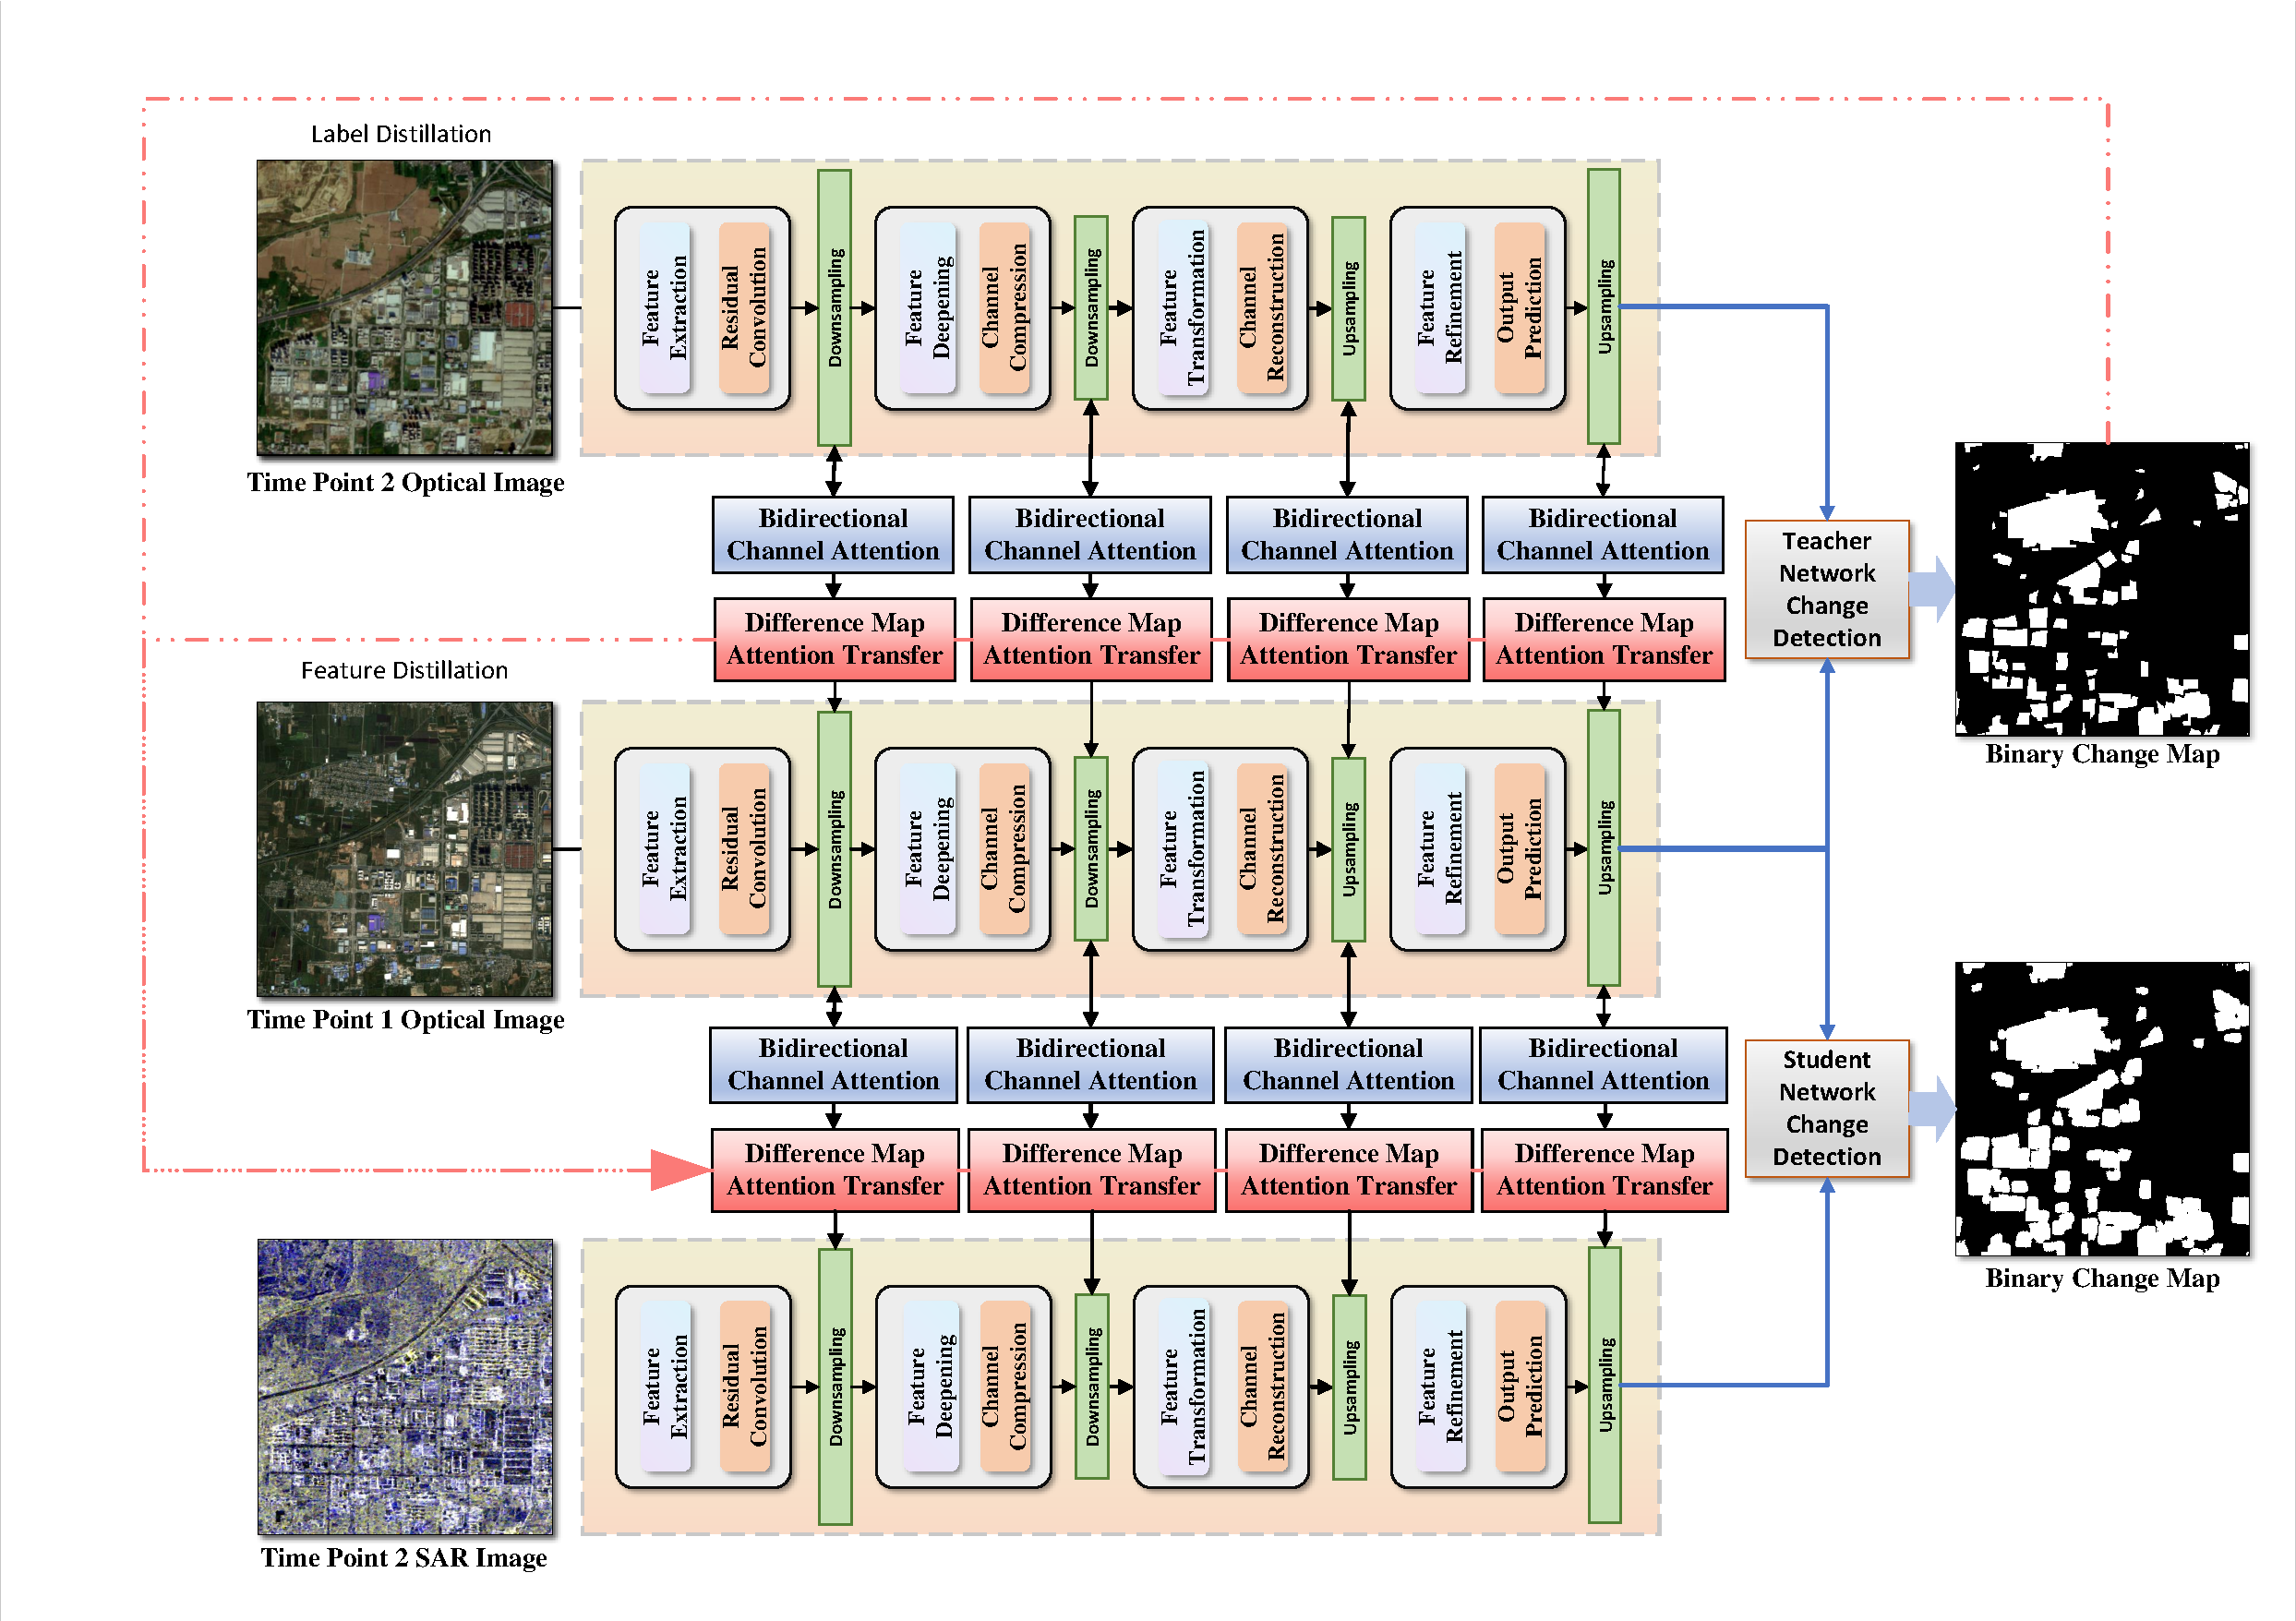
\includegraphics[width=0.9\textwidth]{figures/model_framework.pdf}
\caption{Overall framework of the proposed GOLD model. The three-branch design includes a shared pre-event optical branch, a post-event SAR branch for the student network, and a post-event optical branch for the teacher network.}
\label{fig:model_framework}
\end{figure*}

\subsection{Online Distillation with Multi-level Knowledge Transfer}
Building upon this three-branch design, GOLD introduces an online distillation strategy that enables continuous knowledge transfer from the homogeneous teacher to the heterogeneous student. Unlike conventional distillation, which enforces only output-level consistency, our method enforces alignment across features, outputs, and attentions. This hierarchical formulation ensures that both discriminative cues and structural knowledge are effectively conveyed, thereby enhancing the student’s cross-modal generalization. To achieve this, we construct a set of tailored loss functions that jointly optimize these complementary objectives.    

At the feature level, mean squared error (MSE) and cosine similarity are combined to constrain both value proximity and directional consistency between teacher and student embeddings:
\begin{align}
\mathcal{L}_{feat} = 0.7 \cdot MSE(F_s,F_t) + 0.3 \cdot Cos(F_s,F_t),
\end{align}
where $F_s$ and $F_t$ denote student and teacher features. The weighting prioritizes magnitude alignment while retaining orientation sensitivity, which is critical for heterogeneous feature representation.  

At the output level, Kullback--Leibler divergence is applied to align the softened probability distributions of teacher and student:
\begin{align}
\mathcal{L}_{out} = D_{KL}(S_s,S_t) \cdot T^2,
\end{align}
where $S_s$ and $S_t$ are temperature-scaled outputs and $T$ controls distribution smoothness. A higher $T$ reveals fine-grained knowledge, while the factor $T^2$ compensates for gradient attenuation.  

At the attention level, we introduce difference-map guided distillation that aligns spatial and channel attentions with explicit supervision from difference maps:
\begin{align}
\mathcal{L}_{att\_D} = 0.5 \mathcal{L}_{map} + 0.3 \mathcal{L}_{ch} + 0.2 \mathcal{L}_{sp}.
\end{align}
Here, difference maps are emphasized as the fundamental descriptor of change, channel attention captures \textit{what} has changed, and spatial attention localizes \textit{where} changes occur. This mechanism is detailed in Section~4.3.  

Finally, the three components are integrated as the overall distillation objective:
\begin{align}
\mathcal{L}_D = 0.3 \mathcal{L}_{feat} + 0.4 \mathcal{L}_{out} + 0.3 \mathcal{L}_{att\_D}.
\end{align}
This hierarchical formulation jointly constrains outputs, intermediate features, and attention patterns, thereby reducing modality discrepancies and ensuring effective transfer of discriminative capacity and interpretability from the teacher to the student.

\subsection{Difference Map Attention Transfer: Visual Guide for Change Perception}
While traditional distillation enforces consistency only at the output level, heterogeneous change detection requires alignment of intermediate perceptual cues. To this end, we propose difference map attention transfer, which constructs a modality-robust difference signal, induces complementary attentions, and aligns the student’s perceptual focus with that of the homogeneous teacher.

Given bi-temporal features $F_1$ and $F_2$, we compute a dual-metric difference that captures both magnitude and directional variation. The Euclidean term
\begin{equation}
D_{\mathrm{L2}}=\sqrt{\lVert F_1-F_2\rVert_2^2+\epsilon}
\end{equation}
measures intensity deviations, while the cosine term
\begin{equation}
D_{\mathrm{cos}}=1-\frac{F_1\!\cdot\! F_2}{\lVert F_1\rVert_2\,\lVert F_2\rVert_2+\epsilon}
\end{equation}
captures orientation change, mitigating scale sensitivity. The fused signal is normalized to $[0,1]$ for optimization stability:
\begin{equation}
D=\tanh\!\Big(2\cdot\tfrac{1}{2}(D_{\mathrm{L2}}+D_{\mathrm{cos}})\Big)\cdot 0.5+0.5.
\end{equation}

This difference map drives two complementary attentions. Spatial attention indicates where changes occur by aggregating channel statistics:
\begin{equation}
A_{\mathrm{sp}}=\sigma\!\big(\mathrm{Conv}([\mathrm{Mean}_c(F),\,\mathrm{Max}_c(F)])\big),
\end{equation}
while channel attention identifies what has changed by modeling inter-channel dependencies:
\begin{equation}
A_{\mathrm{ch}}=\sigma\!\big(\mathrm{FC}(\mathrm{AvgPool}_{hw}(F))+\mathrm{FC}(\mathrm{MaxPool}_{hw}(F))\big).
\end{equation}
Their synergy sharpens both spatial localization and semantic discrimination.  

To transfer this perceptual behavior across modalities, the teacher (optical–optical) produces $\{D_t,A_{\mathrm{sp}}^{t},A_{\mathrm{ch}}^{t}\}$, while the student (optical–SAR) produces $\{D_s,A_{\mathrm{sp}}^{s},A_{\mathrm{ch}}^{s}\}$. They are aligned by mean-squared penalties:
\begin{align}
\mathcal{L}_{\mathrm{map}}&=\mathrm{MSE}(D_s,D_t),\\
\mathcal{L}_{\mathrm{sp}}&=\mathrm{MSE}(A_{\mathrm{sp}}^{s},A_{\mathrm{sp}}^{t}),\\
\mathcal{L}_{\mathrm{ch}}&=\mathrm{MSE}(A_{\mathrm{ch}}^{s},A_{\mathrm{ch}}^{t}).
\end{align}
Aggregated across layers, the final loss is
\begin{equation}
\mathcal{L}_{att\_D} = 0.5 \mathcal{L}_{map}+0.3 \mathcal{L}_{ch}+0.2 \mathcal{L}_{sp}.
\end{equation}

This mechanism aligns the student’s perceptual attention with the teacher across modalities, ensuring both accuracy and interpretability: the model highlights the same regions and feature channels as evidence of detected changes.


\section{Experiments and Results Analysis}
This section presents the experimental evaluation of our proposed GOLD model for heterogeneous remote sensing change detection. We describe the experimental setup, dataset details, comparison with state-of-the-art methods, and ablation studies to validate the effectiveness of each component in our approach.

\subsection{Experimental Setup}
\subsubsection{Hyperparameter Settings}
To ensure the reproducibility of our experiments, we provide the detailed hyperparameter settings used for training the GOLD model. The basic training parameters are listed in Table 1.

\begin{table}[htbp]
\centering
\caption{Basic Training Parameters}
\begin{tabular}{lll}
\hline
Parameter Name & Value & Description \\
\hline
Batch Size & 8 & Training batch size \\
Initial Learning Rate & 0.0005 & Starting learning rate \\
Optimizer & AdamW & Training acceleration optimizer \\
Learning Rate Strategy & Cosine Annealing & Smooth learning rate reduction \\
Training Epochs & 400 & Total training epochs \\
Initialization Type & Normal & Weight initialization with gain factor 0.02 \\
\hline
\end{tabular}
\label{tab:basic_params}
\end{table}

For the distillation and attention mechanisms, we carefully selected parameters to ensure effective knowledge transfer between teacher and student networks, as shown in Table 2.

\begin{table}[htbp]
\centering
\caption{Distillation and Attention Parameters}
\begin{tabular}{lll}
\hline
Parameter Name & Value & Description \\
\hline
Distillation Temperature & 2 & Soft label smoothing parameter \\
Feature Distillation Weight & 0.3 & Feature-level distillation loss contribution \\
Output Distillation Weight & 0.4 & Output-level distillation loss contribution \\
Difference Map Attention Weight & 0.3 & Difference map attention loss contribution \\
Difference Map Weight & 0.5 & Weight of difference map loss in attention loss \\
Channel Attention Weight & 0.3 & Weight of channel attention in attention loss \\
Spatial Attention Weight & 0.2 & Weight of spatial attention in attention loss \\
Difference Map Scaling Factor & 10 & Scaling coefficient for total difference map attention loss \\
\hline
\end{tabular}
\label{tab:distillation_params}
\end{table}

Advanced optimization parameters were set to balance training stability, efficiency, and model performance, as detailed in Table 3.

\begin{table}[htbp]
\centering
\caption{Dynamic Weight and Advanced Optimization Parameters}
\begin{tabular}{lll}
\hline
Parameter Name & Value & Description \\
\hline
Warm-up Epochs & 20 & Epochs for transition from fixed to dynamic weights \\
Gradient Clipping Norm & 1 & Clipping threshold to prevent gradient explosion \\
Gradient Accumulation Steps & 1 & Gradient accumulation mechanism for large batch training \\
Bidirectional Attention Mechanism & Enabled & Enhanced modal information flow \\
Contrastive Learning Loss & Enabled & Weight 10.0, temperature parameter 0.5 \\
\hline
\end{tabular}
\label{tab:advanced_params}
\end{table}

\subsubsection{Training Optimization Strategy}
In training deep learning models, the choice of optimizer and learning rate adjustment significantly impacts training effectiveness and convergence speed. Our research employs the AdamW optimizer for parameter updates:

\begin{equation}
\theta_{t+1} = \theta_t - \eta \cdot \frac{\hat{m}_t}{\sqrt{\hat{v}_t}} + \epsilon - \eta \cdot \lambda \cdot \theta_t
\end{equation}

where the learning rate $\eta = 0.0005$ and weight decay coefficient $\lambda = 0.01$. The model is initially trained using pre-trained ResNet-18 weights with a cosine learning rate decay strategy to ensure smooth learning rate reduction during training:

\begin{equation}
\eta_t = \eta_{min} + \frac{1}{2}(\eta_{max} - \eta_{min})(1 + \cos(\frac{t_{current}}{t_{total}}\pi))
\end{equation}

Additionally, we implemented several training optimization strategies: multi-GPU parallel processing to distribute training tasks across multiple GPUs, significantly reducing computation time; data pre-loading using multi-threading to avoid data loading bottlenecks; checkpoint training allowing for saving training states and resuming from saved points when needed; and gradient accumulation to optimize memory usage by accumulating gradients over multiple steps, enabling large-batch effects even with limited memory resources.

\subsection{Dataset Description}
The preprocessed remote sensing images were annotated using our developed LabelmeCD-AI tool. The completed dataset comprises 24 groups, each including a pre-event optical image (A), post-event SAR image (B), post-event optical image (C), and change label. To match the GOLD network structure, we used 512×512 pixel patches with 50\% overlap, generating 2370 patches from the original images. After quality inspection, we removed 208 "all-black" patches with average pixel values below 5.0, resulting in 2162 valid image patches.

To avoid data leakage between training and validation sets, we grouped these overlapping image patches. The original images were divided into 1068 non-overlapping image groups, and the change region ratio (percentage of white pixels in the label image) was calculated for each group. When dividing the dataset, we followed the principle that "different regions of the same original image should not appear in both training and validation sets simultaneously." The training set was allocated 1740 images with an average change region ratio of 6.54\%, accounting for 80.5\% of the total; the validation set received 422 images with an average change region ratio of 6.36\%, containing 395 images and accounting for 19.5\% of the total. During training, in addition to flipping and rotation, we also employed random cropping and scaling, Gaussian blur, and color jittering for data augmentation.

This dataset allocation method addresses issues of inconsistent sizes, varying data quality, and improper dataset division leading to information leakage in heterogeneous remote sensing image processing, providing a well-structured and balanced high-quality dataset for subsequent model training.

\subsection{Comparative Results}
To comprehensively evaluate the advantages of the proposed GOLD model in heterogeneous remote sensing image change detection tasks, we selected several state-of-the-art models widely applied in the literature and compared their performance with the GOLD student network on our custom dataset using the same evaluation metrics.

The comparison models include:

\begin{enumerate}
    \item FC-EF: The most common siamese fully convolutional network model using heuristic methods for change detection.
    \item LightCDNet: A lightweight change detection network designed for industrial applications and edge devices, composed of fusion backbone network and pyramid decoder, with its core component being a deep supervision fusion module that guides early fusion of main features to improve performance. While maintaining high accuracy, it reduces model size, suitable for resource-constrained environments.
    \item TinyCD: A lightweight change detection model using siamese U-Net architecture, leveraging low-level features in a global temporal and local spatial manner, employing a new strategy to mix features in the spatio-temporal domain, and combining MLP blocks to form a spatial-semantic attention mechanism - the mix and attention mask block, achieving excellent change detection performance with minimal model size.
    \item BIT: A model utilizing Transformer for remote sensing image change detection, modeling long-range conceptual relationships in the compact token-based spatiotemporal context by representing bi-temporal images as semantic tokens, using less than three times the computational cost and model parameters compared to pure convolutional baselines.
    \item SNUNet-ECAM: A combination of densely connected siamese network and U-Net, with tight information transmission between encoders and decoders, and between decoders and decoders, reducing the loss of localization information in deep networks. It also introduces an integrated channel attention module for deep supervision, refining representative features at different semantic levels, achieving a good balance between accuracy and computational cost.
    \item ChangeFormer: A more sophisticated Transformer-based siamese network architecture that unifies a hierarchical Transformer encoder with a multi-layer perceptron decoder, efficiently presenting the multi-scale long-distance details required for accurate change detection, excelling in complex scene changes.
\end{enumerate}

\begin{table}[htbp]
\centering
\caption{Experimental Results Comparison}
\begin{tabular}{lllll}
\hline
Model & IoU & F1 & Precision & Recall \\
\hline
FC\_EF & 66.95 & 76.63 & 84.94 & 71.83 \\
LightCDNet & 67.17 & 76.84 & 85.52 & 71.90 \\
ChangerStar & 68.65 & 78.20 & 93.56 & 71.39 \\
TinyCD & 75.32 & 84.22 & 89.31 & 80.44 \\
BIT & 77.25 & 85.87 & 83.16 & 89.18 \\
HeteGAN & 78.21 & 86.74 & 88.32 & 83.65 \\
SNUNet\_ECAM & 81.54 & 88.99 & 91.58 & 86.74 \\
ChangeFormer & 84.21 & 90.83 & 93.98 & 88.16 \\
GOLD (Student) & 85.98 & 92.02 & 90.94 & 93.16 \\
GOLD (Teacher) (Homogeneous) & 86.61 & 92.42 & 90.70 & 94.34 \\
IFN & 87.71 & 93.11 & 93.82 & 92.43 \\
Changer & 88.43 & 93.56 & 95.21 & 92.04 \\
\hline
\end{tabular}
\label{tab:results}
\end{table}

Experimental results in Table 4 show that our proposed GOLD model performs excellently in heterogeneous remote sensing image change detection tasks. In remote sensing image change detection, IoU is the key metric directly reflecting the overlap degree of changed regions. The GOLD student network achieves an IoU of 85.98\% on heterogeneous data, significantly higher than other comparison methods.

Despite dealing with more challenging heterogeneous data, the GOLD student network based on online knowledge distillation performs almost on par with the teacher network on homogeneous data (IoU 85.98\% vs 86.61\%), with only a 0.63\% gap, fully demonstrating the powerful effectiveness of the online knowledge distillation method proposed in this paper. Through the innovative difference map attention transfer mechanism and dynamic weight allocation strategy designed in this paper, the teacher network can efficiently transfer knowledge of homogeneous data processing to the student network in real-time during training, enabling the student network to effectively address modal differences and feature inconsistency problems in heterogeneous data.

In contrast, other models have various shortcomings. The state-of-the-art ChangeFormer has an IoU of 84.21\%, nearly 2 percentage points lower than our GOLD student network. SNUNet\_ECAM also performs well with an IoU of 81.54\%, but still significantly lags behind our model. BIT performs well in recall (89.18\%) but has an overall IoU of only 77.25\%. The weaker FC\_EF and LightCDNet have IoUs of 66.95\% and 67.17\% respectively, far inferior to the GOLD model in detecting changes in complex scenes.

The excellent performance of the GOLD model is primarily attributed to the online knowledge distillation mechanism. Unlike traditional pre-training-fine-tuning or offline distillation, the online distillation method allows the teacher and student networks to train simultaneously, achieving real-time knowledge transfer. The difference map attention transfer mechanism allows the GOLD teacher network to directly use high-quality change features extracted from homogeneous data to guide the student network, helping the student network accurately locate changed regions in heterogeneous data. This innovative learning approach not only significantly improves model performance in heterogeneous remote sensing change detection tasks but also provides new ideas for solving data heterogeneity problems commonly encountered in the remote sensing field.

\subsection{Ablation Studies}
\begin{table}[htbp]
\centering
\caption{Impact of Different Components on Model Performance}
\begin{tabular}{lllll}
\hline
Model Configuration & IoU & F1 & Precision & Recall \\
\hline
Baseline Model & 78.21 & 86.74 & 88.32 & 83.65 \\
+Three-Branch Online Distillation & 83.12 & 90.34 & 89.21 & 90.23 \\
+Difference Map Attention Transfer & 84.21 & 90.83 & 89.58 & 91.14 \\
+Dynamic Weight Allocation (Complete) & 85.98 & 92.02 & 90.94 & 93.16 \\
-Lightweight Model & 82.84 & 89.55 & 87.59 & 90.79 \\
\hline
\end{tabular}
\label{tab:ablation}
\end{table}

To comprehensively evaluate the effectiveness of each component in our proposed method, we conducted a series of ablation studies. From Table 5, it is evident that the three-branch online distillation strategy brings significant performance improvements, with precision increasing from 88.32\% to 89.21\%, recall dramatically increasing from 83.65\% to 90.23\%, and IoU improving from 78.21\% to 83.12\%, an increase of about 4.91 percentage points. This demonstrates that when dealing with heterogeneous remote sensing image change detection tasks, using the teacher network (optical-optical branch) to guide the student network (optical-SAR branch) through knowledge distillation is highly effective.

After introducing the difference map attention transfer mechanism, the model's precision improved to 89.58\%, recall reached 91.14\%, and IoU reached 84.21\%, an increase of about 1.09 percentage points compared to the model using only distillation. This indicates that difference map attention transfer enhances the model's perception ability for changed regions by focusing on key features in image change areas, reducing false positives and false negatives.

Finally, the addition of the dynamic weight allocation mechanism brings the complete model's performance to its optimum, with precision improved to 90.94\%, recall reaching 93.16\%, F1 value reaching 92.02\%, and IoU improved to 85.98\%, an additional increase of about 1.77 percentage points from the previous stage. Dynamic weight allocation adaptively adjusts the weights of different loss items according to their importance in the training process, balancing change detection loss, distillation loss, and attention loss contributions, avoiding dominance by a single loss item, thus enabling the model to learn change features in heterogeneous images more comprehensively.

\begin{table}[htbp]
\centering
\caption{GPU Resource Usage Comparison between GOLD Complete and Lightweight Models}
\begin{tabular}{llll}
\hline
Model Type & Parameters (M) & GPU Memory (MB) & GPU Energy Rate (\%) \\
\hline
Complete Model & 37.254 & 6319.8 & 20 \\
Lightweight Model & 9.401 & 2571.8 & 3.8 \\
\hline
\end{tabular}
\label{tab:resource_usage}
\end{table}

Our research also explored the trade-off between model complexity and performance, designing a lightweight version of the model. As seen in Table 6, compared to the complete model's 37.254M parameters, the lightweight model significantly reduces computational complexity through a series of core strategies while maintaining high detection performance with only 9.401M parameters. For the backbone network, the number of channels in the main convolutional layers is reduced by 50\% (from 128 to 64), some 3×3 convolutions are replaced with 1×1 convolutions to reduce parameter count, and some residual connections are reduced. For attention modules, the reduction ratio is increased from 16 to 32, the MLP layer structure is simplified, and the number of intermediate channels is reduced. For feature fusion optimization, some feature concatenation operations are replaced with computationally cheaper weighted sum operations, and the number of channels in pre-fusion transformation layers is reduced. The distillation process is also streamlined by selectively transmitting only key layer feature information for distillation, optimizing the distillation temperature parameter to improve knowledge transfer efficiency, and simplifying the teacher network structure while maintaining key feature representation capability. Although the lightweight model's precision decreases to 87.59\%, it maintains performance close to the complete model (IoU decreased from 85.98\% to 82.84\%) while reducing parameters by about 74.77\%, bringing significant GPU resource savings. The complete model uses an average of 6319.80MB GPU memory during inference, while the lightweight model requires only 2571.80MB, a reduction of about 59.30\%. For GPU energy rate, the complete model averages 20.00\%, while the lightweight model is only 3.80\%. These data fully demonstrate that the lightweight strategy significantly reduces computational resource requirements while maintaining model performance, providing a feasible solution for deployment in edge computing devices and resource-constrained scenarios.

\section*{Acknowledgement}
This work was supported by the National Natural Science Foundation of China under Grant 62471394 and U21B2041, and the Innovation Foundation for Doctoral Dissertation of Northwestern Polytechnical University under Grant CX2024108.

%% Loading bibliography style file 
%\bibliographystyle{model1-num-names}
\bibliographystyle{model5-names}

% Loading bibliography database
\bibliography{cas-refs}


%\vskip3pt


\end{document}

